\documentclass[12pt]{article}
\usepackage[utf8]{inputenc}
\usepackage[a4paper,margin=1in]{geometry}
\usepackage{amsmath} 
\usepackage{amssymb}
\usepackage{graphicx}
\usepackage{float}
\usepackage{tabularx} 
\usepackage{caption}
\usepackage{subcaption}
\usepackage{array}
\usepackage{listings}
\usepackage{pythonhighlight}



\title{
    Department Of Aerospace Engineering,\\
    Indian Institute Of Technology Madras
    \begin{figure}[H]
        \centering
        
\includegraphics[width=8cm]{iitmlogo.png}
    \end{figure}
    \begin{center}
        \textbf{\\AS2101 : Introduction to Aerospace Engineering\\}
        Report 3 : Prime Factor Frequency Distribution\\
    \end{center}
}
\author{
    Pranit Zope\\AE20B046
}
\date{September 6, 2021}

\begin{document}
\pagenumbering{gobble}
\maketitle
\newpage
\pagenumbering{arabic}
\tableofcontents 
\listoffigures

\newpage

\section{Aim}
   To find prime factorisation of each number between 2 and 1000, calculate the frequency of each prime and plot a frequency distribution plot.

\section{Theory}
    We did our procedure in 3 different steps which will be expalained below.
    \subsection{Step 1 : Finding the Least Prime Factor of the number}
        For this technique, we will start with the first number and using divisibility, we will check which us the least prime factor of the number. Then we defined an array "arr[]" and stored the value of the least prime factor of number n as arr[n].\\
        Also since, 0 and 1 have no prime factors, the value of arr[] and arr[] are both 0s.
    
    \subsection{Step 2 : Finding all the prime factors of a number}
        We already have obtained the least prime factor of all numbers from 2 to 1000. Now, to factorise, we repeatedly divide the number by its least prime factor until we obtain 1. For example, prime factorisation of 30 is as follows.
        
        For 30, $k(30)=2$\\
        \begin{equation*}
            \frac{30}{2}=15 ; k(15) = 3
        \end{equation*}
        \begin{equation*}
            \frac{15}{3}=5 ; k(5) = 5
        \end{equation*}
        \begin{equation*}
            \frac{5}{5}=1 ; k(1)=1
        \end{equation*}
        \\Hence,  the prime factorisation of 30 is $2 \times 3 \times 5$\\
        \textit{Here, $k(n)$ is the least prime factor of n}
     
     \subsection{Step 3 : Plotting Frequency distribution}
        \subsubsection{Creating a list of primes array}
            Until now, we can conclude that the numbers who have only 2 factors (i.e. 1 and itself) are prime. This can lead us up to the conclusion that $k(n) = n$ for all prime numbers.
            So, now we make an array of numbers such that it contains only those numbers which satisfy $k(n)=n$.
        \subsubsection{Creating a frequency array}
            Now for the frequency array, we count how many times a particular number is a prime factor of all numbers.
            We create a variable and increase it every time it occurs in the list of prime factors of a particular number.
        \subsubsection{Plotting both the arrays}
            We use the python library matplotlib.pyplot to plot the given data.\footnote{Code attached in Appendix}  We will make 3 plots, from 2-200, 200-1000 and then the entire plot, 2-1000.
        
\section{Result of Plots}
    \subsection{Plot 1 : 2-200}
        We now plot a figure using our data from Prime numbers array on x axis and data from the Frequency array on y axis.
        We get the following plot. (Fig \ref{fig:2-200})
        \begin{figure}[H]
            \centering
            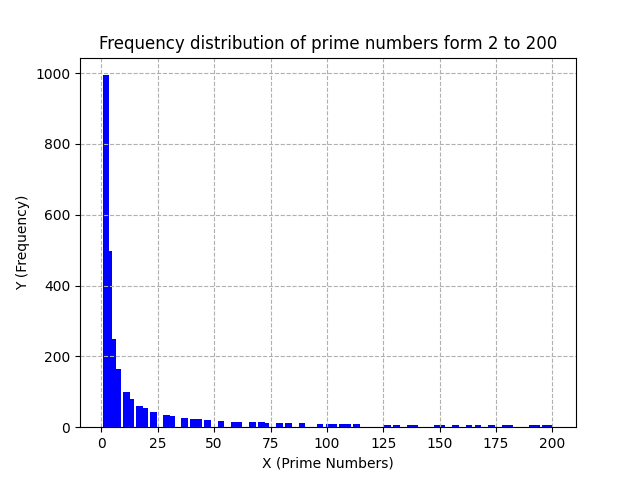
\includegraphics[width=15cm]{fig_2_200.png}
            \caption{Frequency Distribution of Prime factors from 2 to 200}
            \label{fig:2-200}
        \end{figure}
    \newpage
    \subsection{Plot 2 : 201-1000}
        We now plot a figure using our data from Prime numbers array on x axis and data from the Frequency array on y axis.
        We get the following plot. (Fig \ref{fig:201-1000})
        \begin{figure}[H]
            \centering
            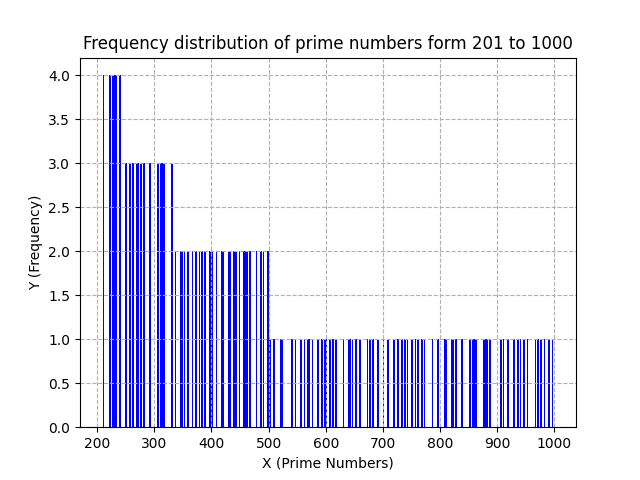
\includegraphics[width=15cm]{fig_201_1000.png}
            \caption{Frequency Distribution of Prime factors from 201 to 1000}
            \label{fig:201-1000}
        \end{figure}   
    \newpage
    \subsection{Plot 3 : 2-1000}
        We now plot a figure using our data from Prime numbers array on x axis and data from the Frequency array on y axis.
        We get the following plot. (Fig \ref{fig:2-1000})
        \begin{figure}[H]
            \centering
            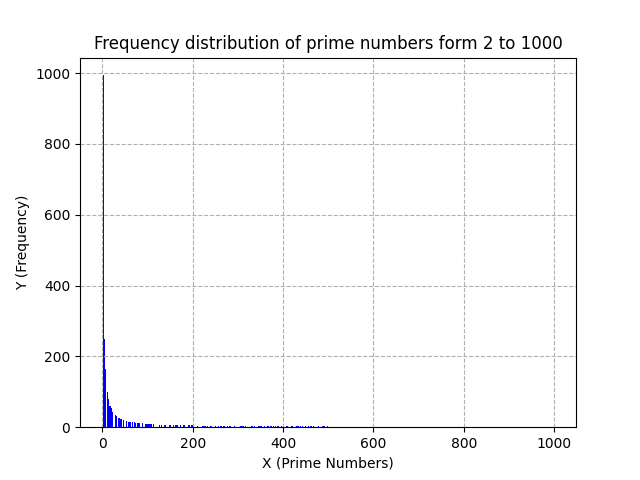
\includegraphics[width=15cm]{fig_2_1000.png}
            \caption{Frequency Distribution of Prime factors from 1 to 1000}
            \label{fig:2-1000}
        \end{figure}
        
\section{Observations}
    We observe that the frequency of prime factors exponentially drops as the number increases.\\ 
    It is 994 at 2 and just 4 at 50. The larger primes above 500 have just a small frequency of 1.\\
    The slope steeply decreases from 0 to 50 and then becomes very less.\\
    At the end, form the 201-1000 plot (Fig \ref{fig:201-1000} we can see that the plot becomes like a step function.

\newpage
\appendix
\addcontentsline{toc}{section}{Appendix}

\section{Python code for computing and plotting frequency distributions}
\begin{python}
# Pranit Zope
# AE20B046
# AS2101 : Assignment 03

import numpy as np
import matplotlib.pyplot as plt

# importing necessary libraries


arr=np.zeros(1001)  # arr will be our array that will have the least prime factor for each number,i.e arr[n] = least prime factor of n

for i in range(1001):
    arr[i]=i
# we first give each element of the array its own value

for i in range(2,1001):
    if(arr[i]==i):
        j=i*i
        while(j<1001):
            if(arr[j]==j):
                arr[j]=i
            j=j+i
# here, we check if our assumption was correct, if not, we correct it and so on, finally we get the array of the least prime factors of numbers


def primefactor(n):
    """A function to return all the prime factors of a given number 'n'.

    Args:
        n (int): The number of which prime factors you want

    Returns:
        factors [array]: An array consisting of all the prime factors of the number
    """

    factors=[]            
    while(n!=1):
        factors.append(arr[int(n)])
        n=n//arr[int(n)]
    return factors



pfct=[] # pfct is an array which will store the prime factors of any number in the form of another array
# eg ; pfct[12]=[2,2,3]

pfct.append(0)
pfct.append(0)
# since 0 and 1 have no prime factors, we will simply write 0 in their place


for i in range(2,1001):
    pfct.append(primefactor(i))
# and pfct = [0],[1],[2],[3],[2,2],[5],[2,3] and so on

for i in range(2,1001):
    print("Prime factors of",i,"are",end=" ")
    for x in pfct[i]:
        print(x,end=",")
    print("\n")
# We print the prime factors of all numbers

pfreq=np.zeros(1001) # pfreq will be the array that contains the frequency of each prime number,  that his how many times it occurs in the prime factorisation of all numbers

for i in range(2,1001):
    for j in pfct[i]:
        pfreq[int(j)]=pfreq[int(j)]+1

A=[]
for i in range(2,1001):
    if(arr[i]==i):
        A.append(int(i))

B=[]
for i in A:
    B.append(int(pfreq[i]))

# We make 2 arrays and store the values of primes and thier frequencies for further use

for i in range(0,len(A)):
    print("Frequency of",A[i],"is:",B[i])

def plot(start,end):
    """A function to plot the frequency distribution plot of prime numbers between a "start" value and "end" value.

    Args:
        start (int): The value at which the plotting needs to begin.
        end (int): The value at which the plotting needs to end.
    """
    x=[]
    for i in A:
        if(i>=start and i<=end):
            x.append(int(i))
        

    y=[]
    for i in x:
        y.append(int(pfreq[i]))
    
    plt.figure()
    plt.grid(linestyle='--')
    plt.title("Frequency distribution of prime numbers form "+str(start)+" to "+str(end))
    plt.xlabel('X (Prime Numbers)')
    plt.ylabel('Y (Frequency)')

    plt.bar(x,y,color='blue',width=3)

    plt.savefig("fig_"+str(start)+"_"+str(end)+".png")
    plt.clf()

# finally, we will plot the required plots
plot(2,1000)
plot(2,200)
plot(201,1000)



\end{python}



\end{document}
